\part{Analysis of Searching}  
\label{ch:effsearch}

\chapter{Searching, binary search trees} %------------------------------------

\section{Table ADT}
\begin{Definition}
A \defnfont{table} is an ADT that supports operations to insert, retrieve and delete an element
with given search key.  Another name is \defnfont{dictionary}.
\end{Definition}
Tables are used for databases. There are  many ways in which a table could be implemented;
with an unsorted list, with a sorted list, with a (balanced) binary search tree, with a hash table.

\section{Sequential search}

In a list with no other structure, the only way to find an element is to 
check each element. 
This takes time in $\Theta(n)$ for any reasonable implementation (such as 
array or linked list).

We only need to be able to iterate through the elements in linear time, so
 even more general structures than lists also allow for this type of search.


\section{Binary search}

In a sorted list where constant time access is possible 
(such as an array implementation), we can find a key $K$ as follows: start at the middle element $y$, and recursively go left (right) if $y>K$ (if $y<K$);
 stop if we hit  $K$ or search subinterval is empty.

Note: binary search is conceptually easy but surprisingly hard to program
 correctly even for professionals (see J. Bentley, \emph{Programming Pearls}).

The (worst-case) recurrence for the running time is $T(n) = 1 +  T(\lfloor n/2 \rfloor)$, with 
solution in $\Theta(\log n)$. The best case is when we find the element on the first try (it is in the middle position).

The execution of this algorithm (looking for all possible keys) can be 
described by a decision tree called a (static) \defnfont{binary search tree}. The 
number of comparisons required to find the key is the depth of the leaf 
containing that key.


\begin{algorithm}[H]
  \caption{Binary search
    \label{alg:binsearch}}
\begin{algorithmic}[1]
%\Require{$0 \leq i \leq j \leq n-1$}
\Function{binsearch}{sorted list $a[0..n-1]$, key $K$}
	\State $L \gets 0$
	\State $R \gets n-1$
	\While{$L \leq R$}
		\State $m \gets \lfloor (L+R)/2\rfloor$ \Comment{median index}
		\If{$A[m] < K$}
			\State $L\gets m+1$
		\ElsIf{$A[m] > K$} 
			\State $R\gets m-1$
		\Else 
			\State \Return $m$ \Comment{key present at index $m$}
		\EndIf
	\EndWhile
	\Return $-1$ \Comment{key not present in list}
\EndFunction
\end{algorithmic}
\end{algorithm}

\section{Binary search trees}
\begin{Definition}
A {binary search tree} (BST) is a binary tree with keys stored in nodes, 
such that the key of each node is $\geq$ the key of every node in the left subtree and $\leq$ 
the key of  every node in the right subtree.
\end{Definition}


A BST implements the Table ADT. To find/insert a key, use binary search as 
described above. To remove a node, we need more work:
\begin{itemize}
\item A node with no children: simply delete.
\item A node with only one child: delete the node, connect the child 
to the parent.
\item A node $n$ with two children: find the minimum key $K$ in the 
right subtree, delete that node, and replace the key of $n$ by $K$.
\end{itemize}

\begin{Boxample}[1] \label{eg:bstDeleteRight}
Follow the above steps to delete node $11$ in the BST shown.\\
\newline
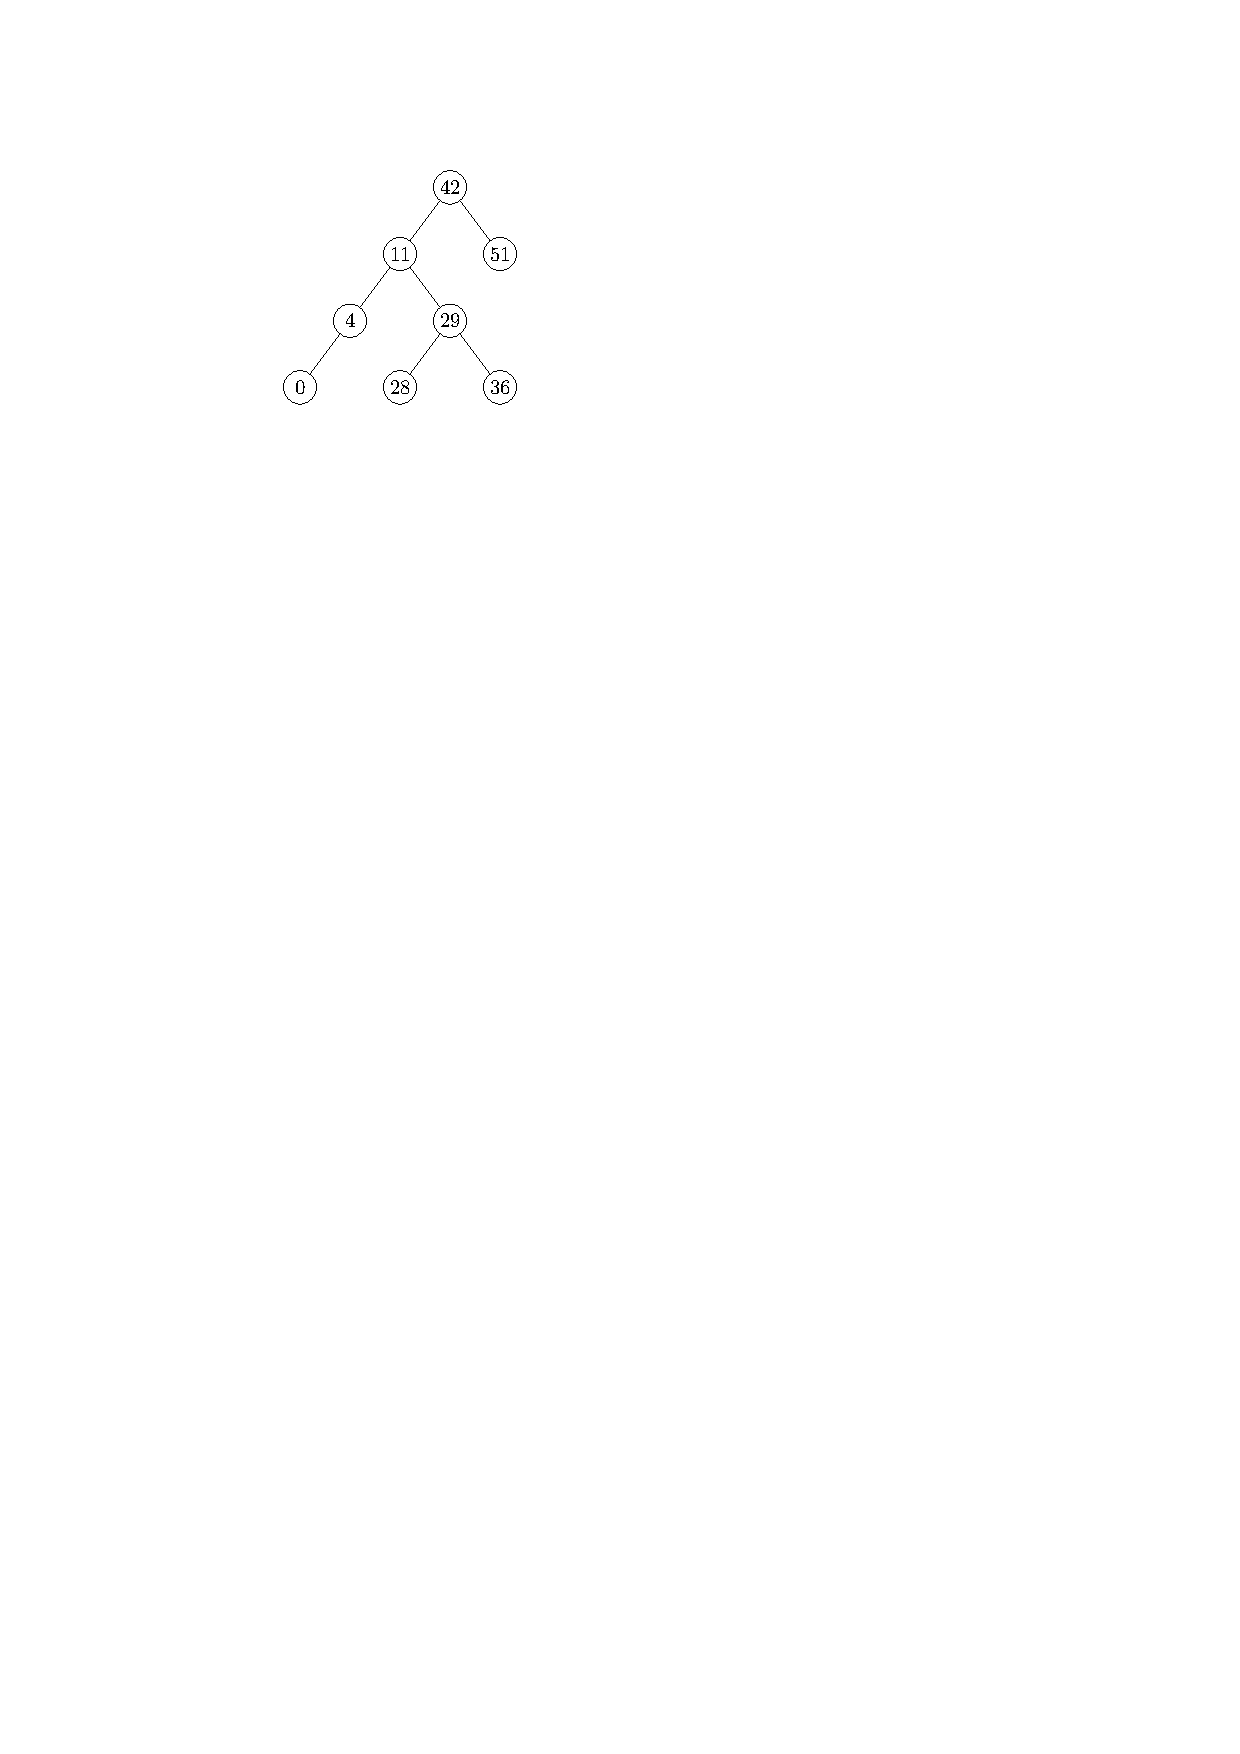
\includegraphics{bstEx}
\end{Boxample}


\section{Analysis of BST operations}

The running time of all basic operations is proportional to the number of 
nodes visited. In the worst case, finding/removing/inserting take time in $\Theta(h)$ 
where $h$ is the height of the tree. Unfortunately the height can be as large 
as $n-1$ in the worst case. Conclusion: we need another idea to guarantee good worst-case 
performance. We need to \emph{rebalance} BSTs.

\begin{Boxample}[5] \label{eg:bstDeleteLeft}
When deleting a node  in a BST, what if we use the maximum key in the left subtree instead?
Carry this out for node $11$ in the BST shown in Example \ref{eg:bstDeleteRight}.

\end{Boxample}


The above example shows that if for deletion we instead use choose the maximum key in the left subtree, everything proceeds as expected. 
However always using the same side can lead to unbalance. Alternating sides, or choosing a side randomly, will more likely  result in a more 
balanced tree.


\section{Treesort}

As we did with heapsort, we can build a binary search tree from our initial list, by inserting elements one at a time. 
We can recover the sorted list by reading the keys according to an inorder traversal (see \cref{fig:inorderTraversal}). 
This takes time in $\Theta(n \log n)$.

As with heapsort, we can do this in place in an array. This is basically quicksort!

\begin{figure}[htb]
  \centering
  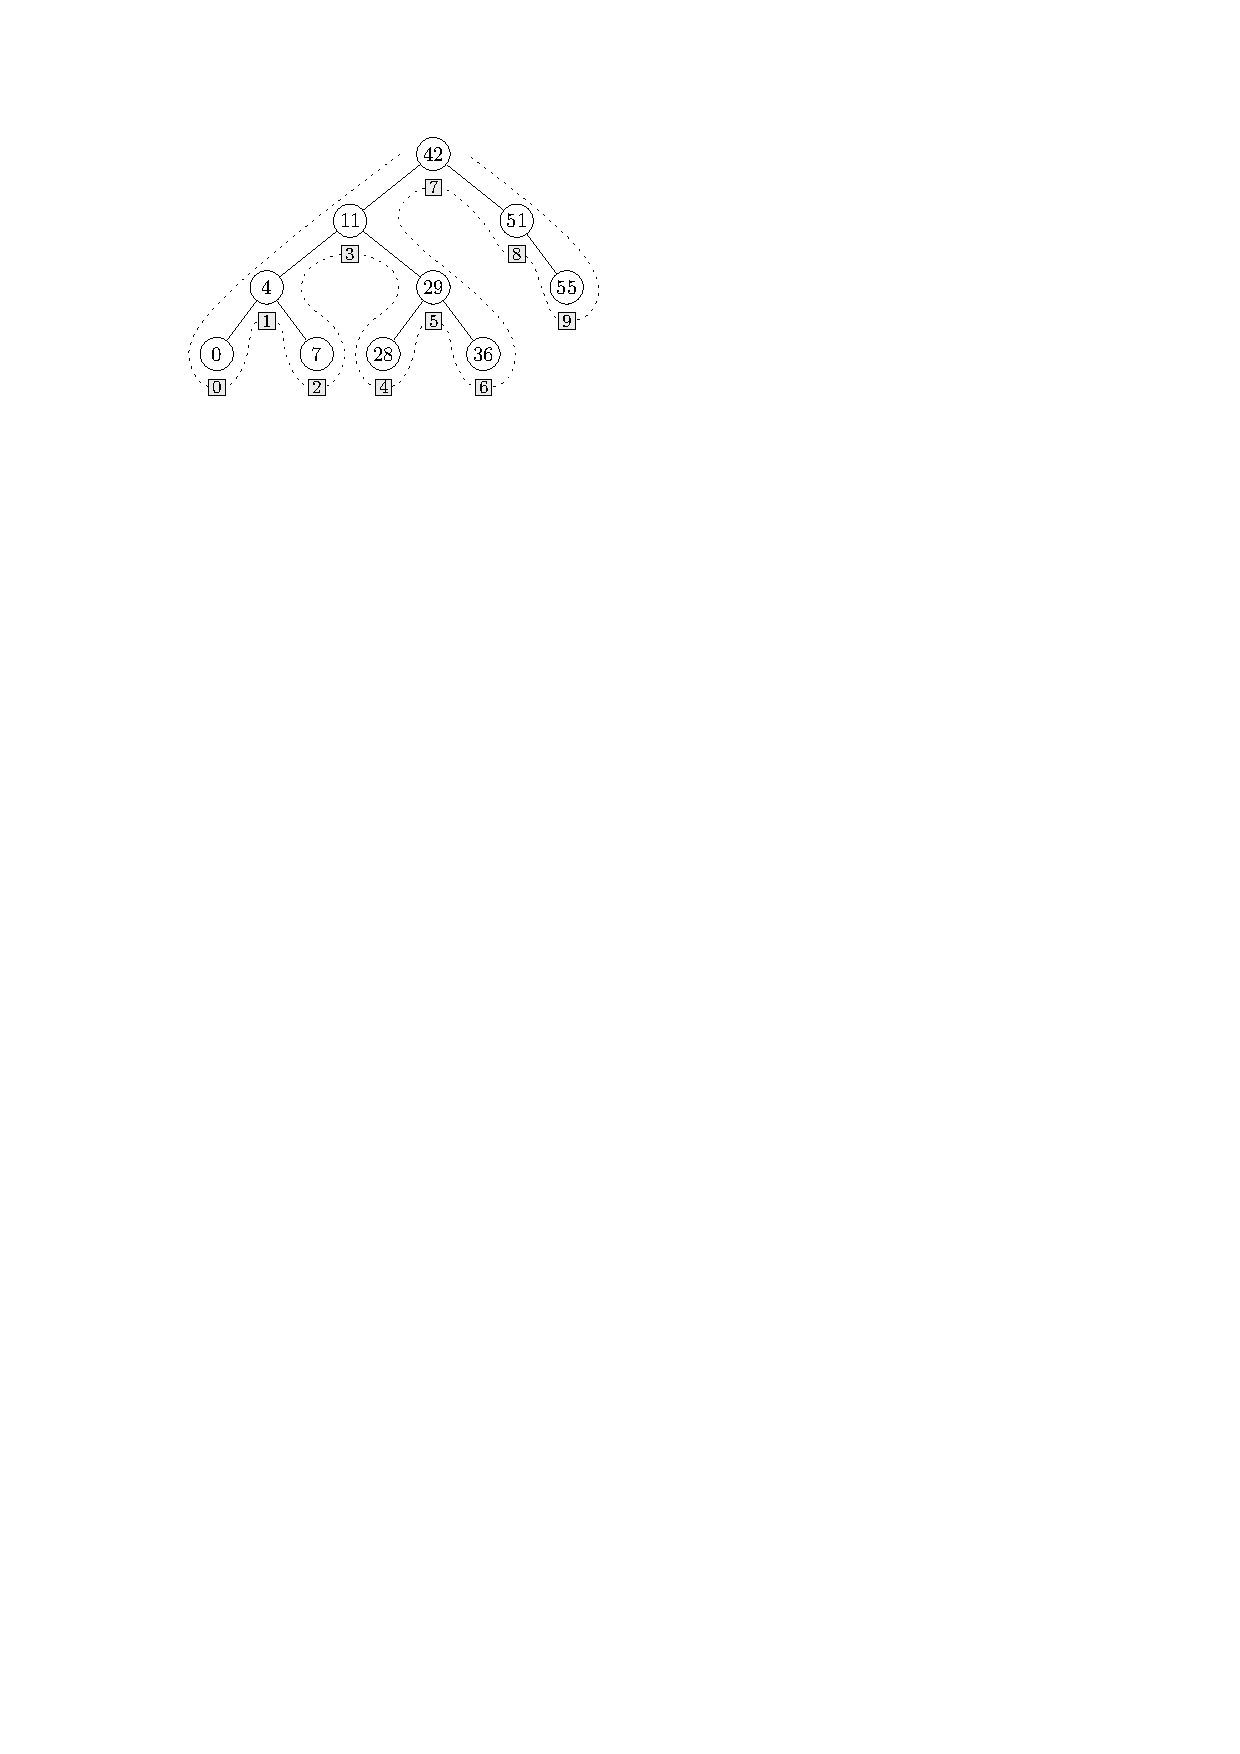
\includegraphics{inorderTraversal}
  % 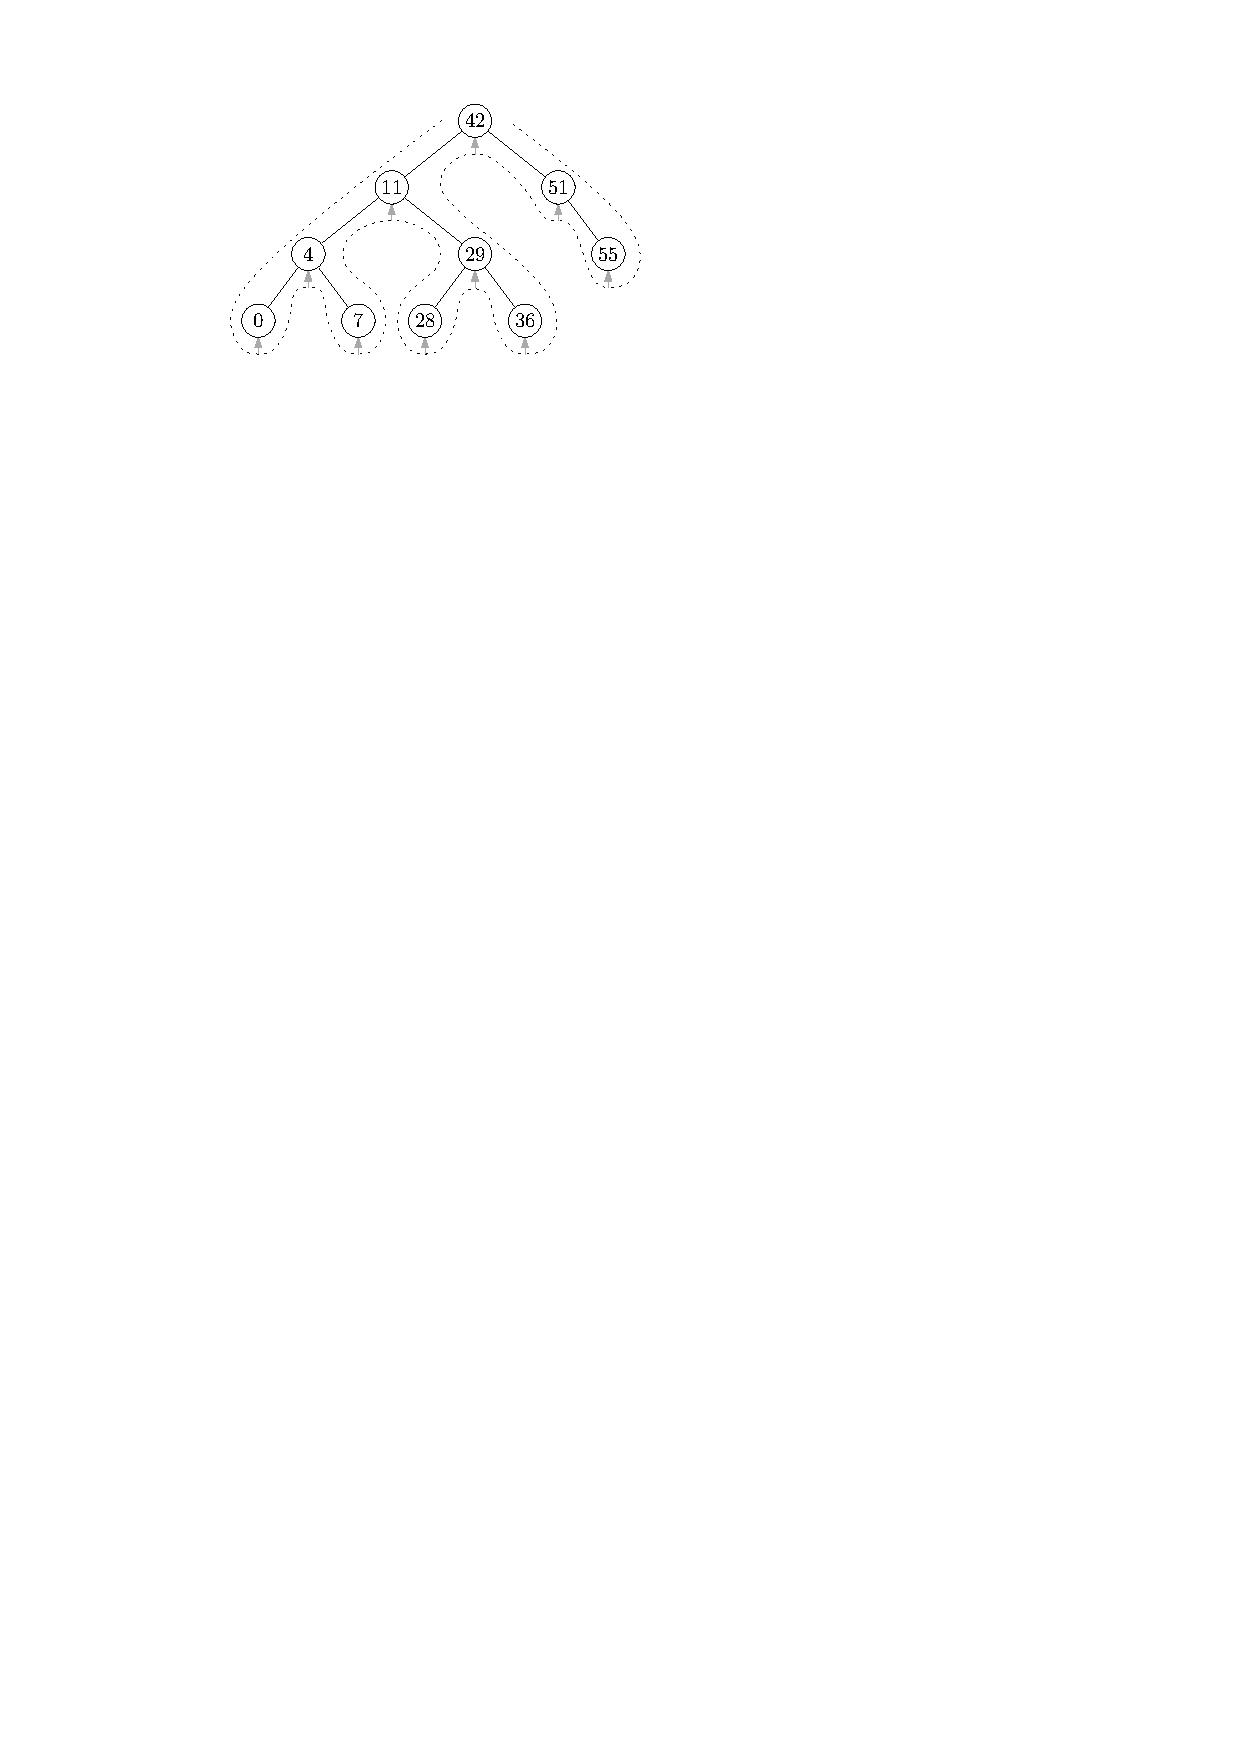
\includegraphics{inorderTraversal2} % alternative version with arrows
  \caption{An inorder traversal of a BST.}
  \label{fig:inorderTraversal}
\end{figure}


\section{Relation between Quicksort and BSTs}

After choosing the pivot and partitioning, we can represent the array as a 
binary tree: pivot at the root, left subfile on the left, right subfile on the 
right. It has the BST property with respect to the sort keys.

Given the above BST describing the execution of quicksort on the array, 
note that the cost of constructing the tree (measured by key comparisons) is 
the same as the number of comparisons used by quicksort in sorting the file.
This is equal to the {internal path length}, the sum of all depths of nodes.

\begin{figure}[htb]
  \centering
  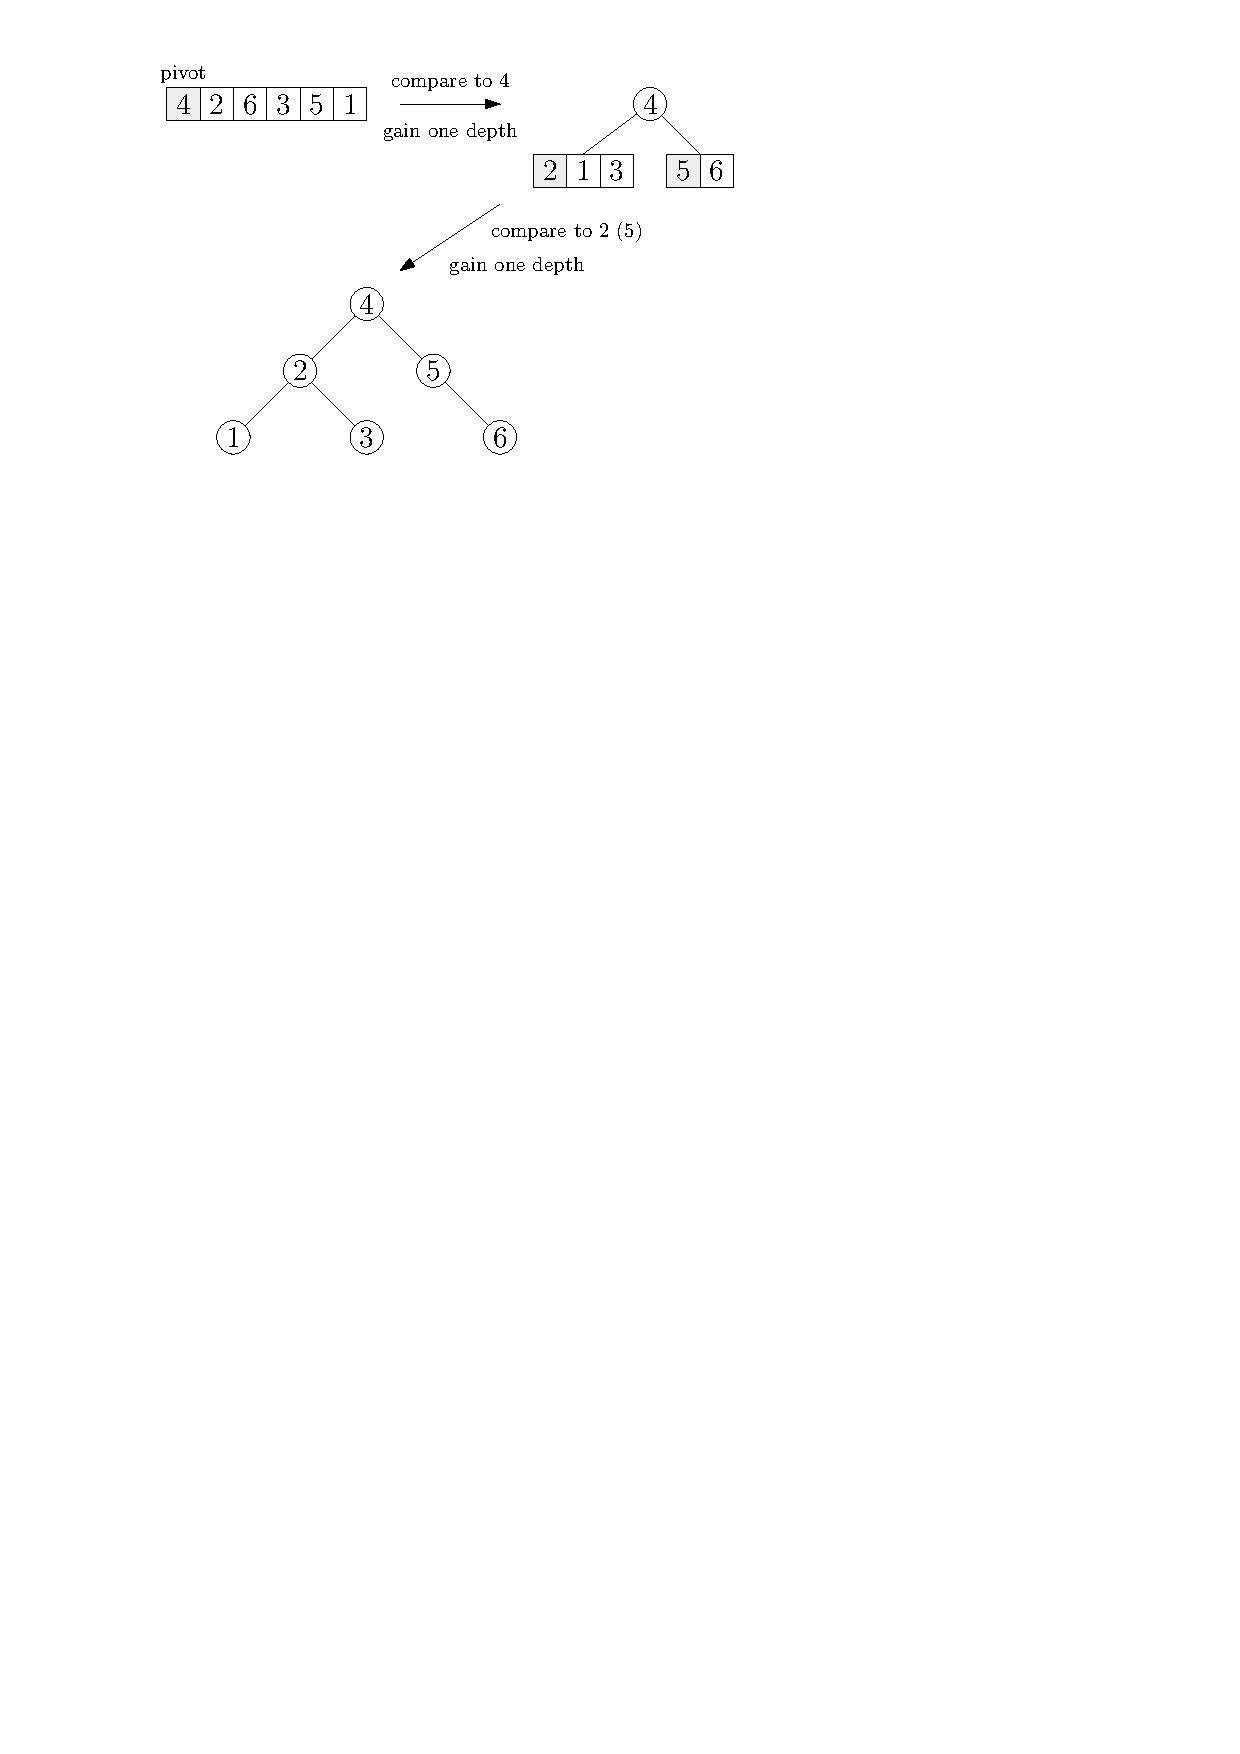
\includegraphics{bstQuicksort}
  \caption{Illustration of the relation between quicksort and BSTs.}
  \label{fig:bstQuicksort}
\end{figure}

Thus the average search cost in a BST built by random insertions is $\Theta(\log n)$ .

% Jo says: I assume you wanted a figure for the relation, because average is hard to illustrate  





\chapter{Self-balancing binary search trees} %--------------------------------
\label{sec:balanced}

There are several classes of BSTs (such as AVL, red-black, AA) that 
perform rebalancing operations at crucial times in order to keep the height 
close to $\lg n$.
These operations are based on local \emph{rotations} of the tree.
Analysis of performance is fairly difficult.
The average-case height is not really known.

\begin{figure}[htb]
  \centering
  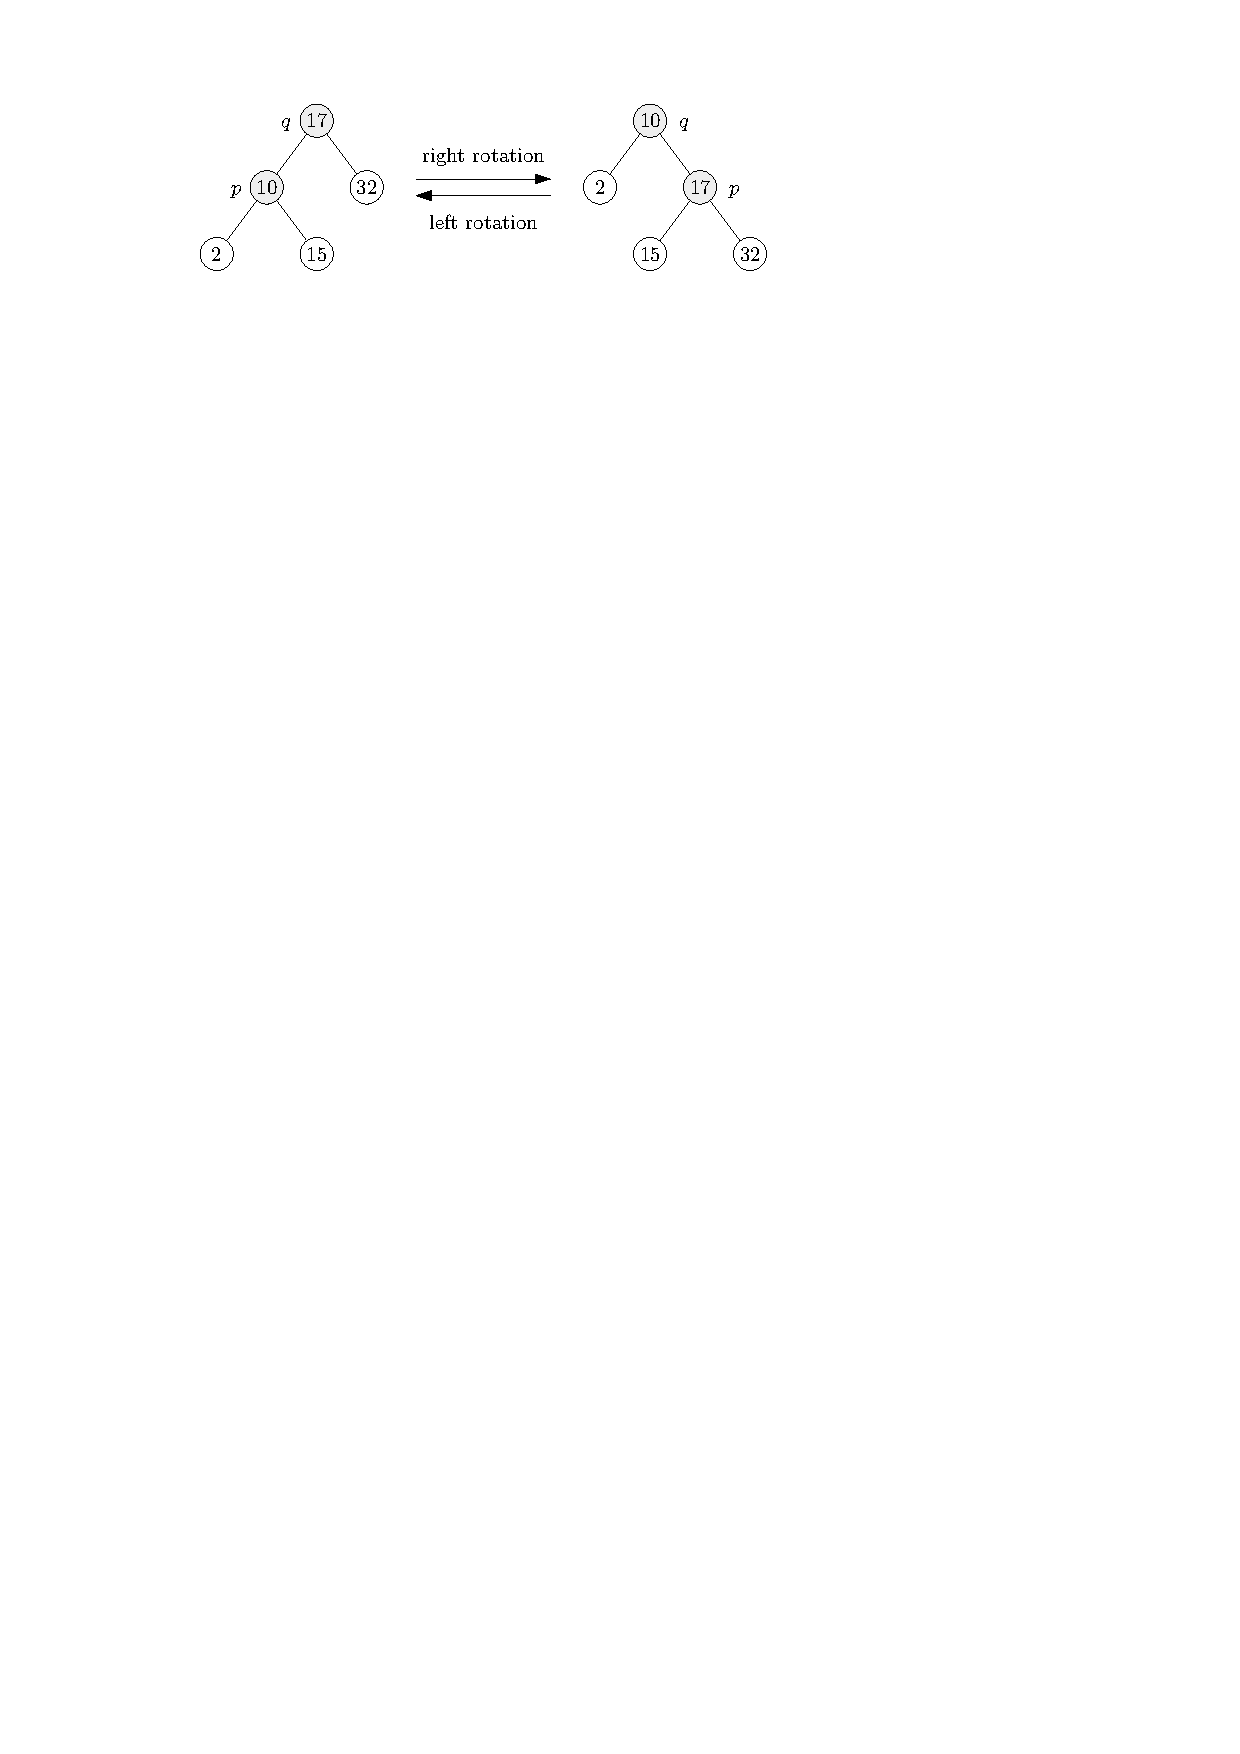
\includegraphics{rotationNumbers}
  %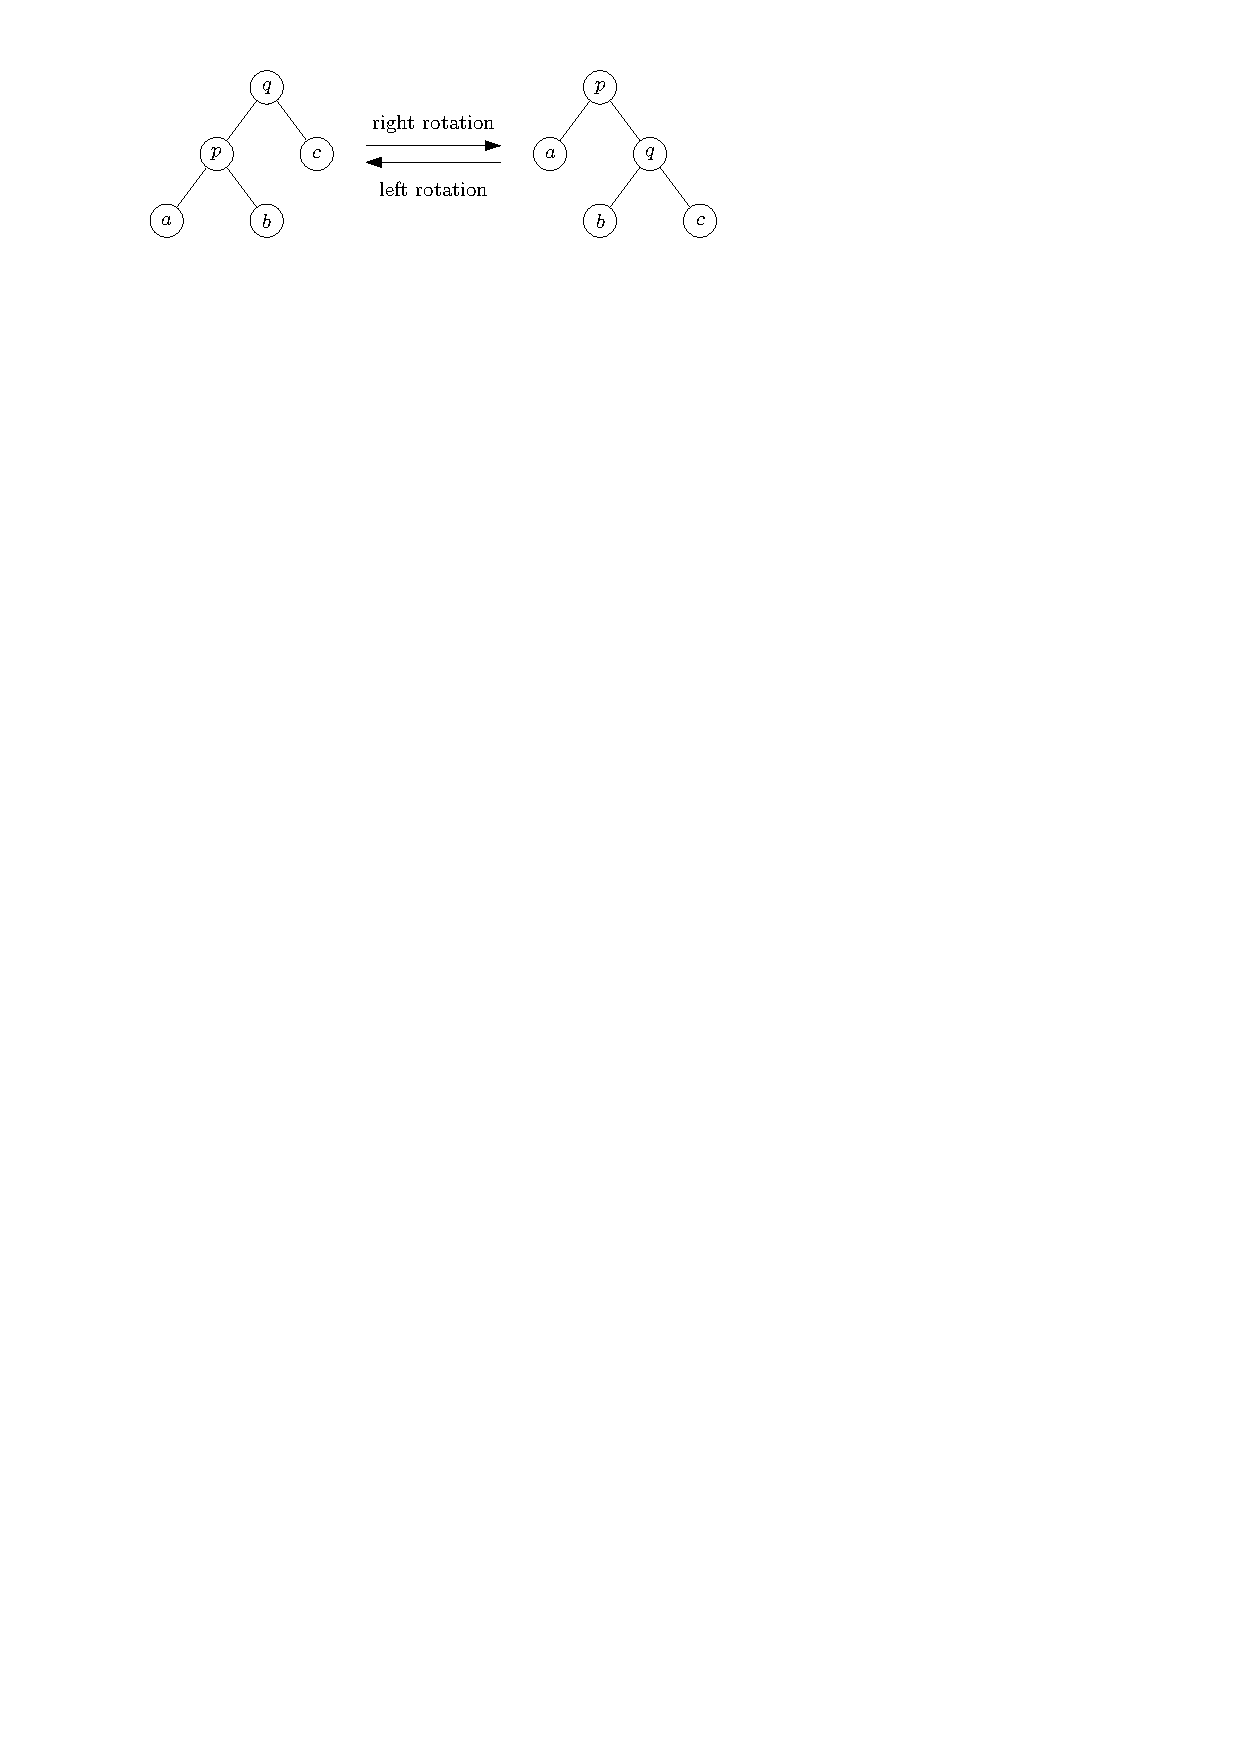
\includegraphics{rotationVariables} % alternative with p, q, a, b, c instead of numbers 
  \caption{Right and left rotation of a BST.}
  \label{fig:rotation}
\end{figure} 

\begin{Boxample}[7]
Perform a right rotation on the BST around the vertices $p = 50$ and $q = 74$ like in \cref{fig:rotation}.
Then perform a left rotation on the resulting BST around the vertices $12$ and $50$.\\
\newline 
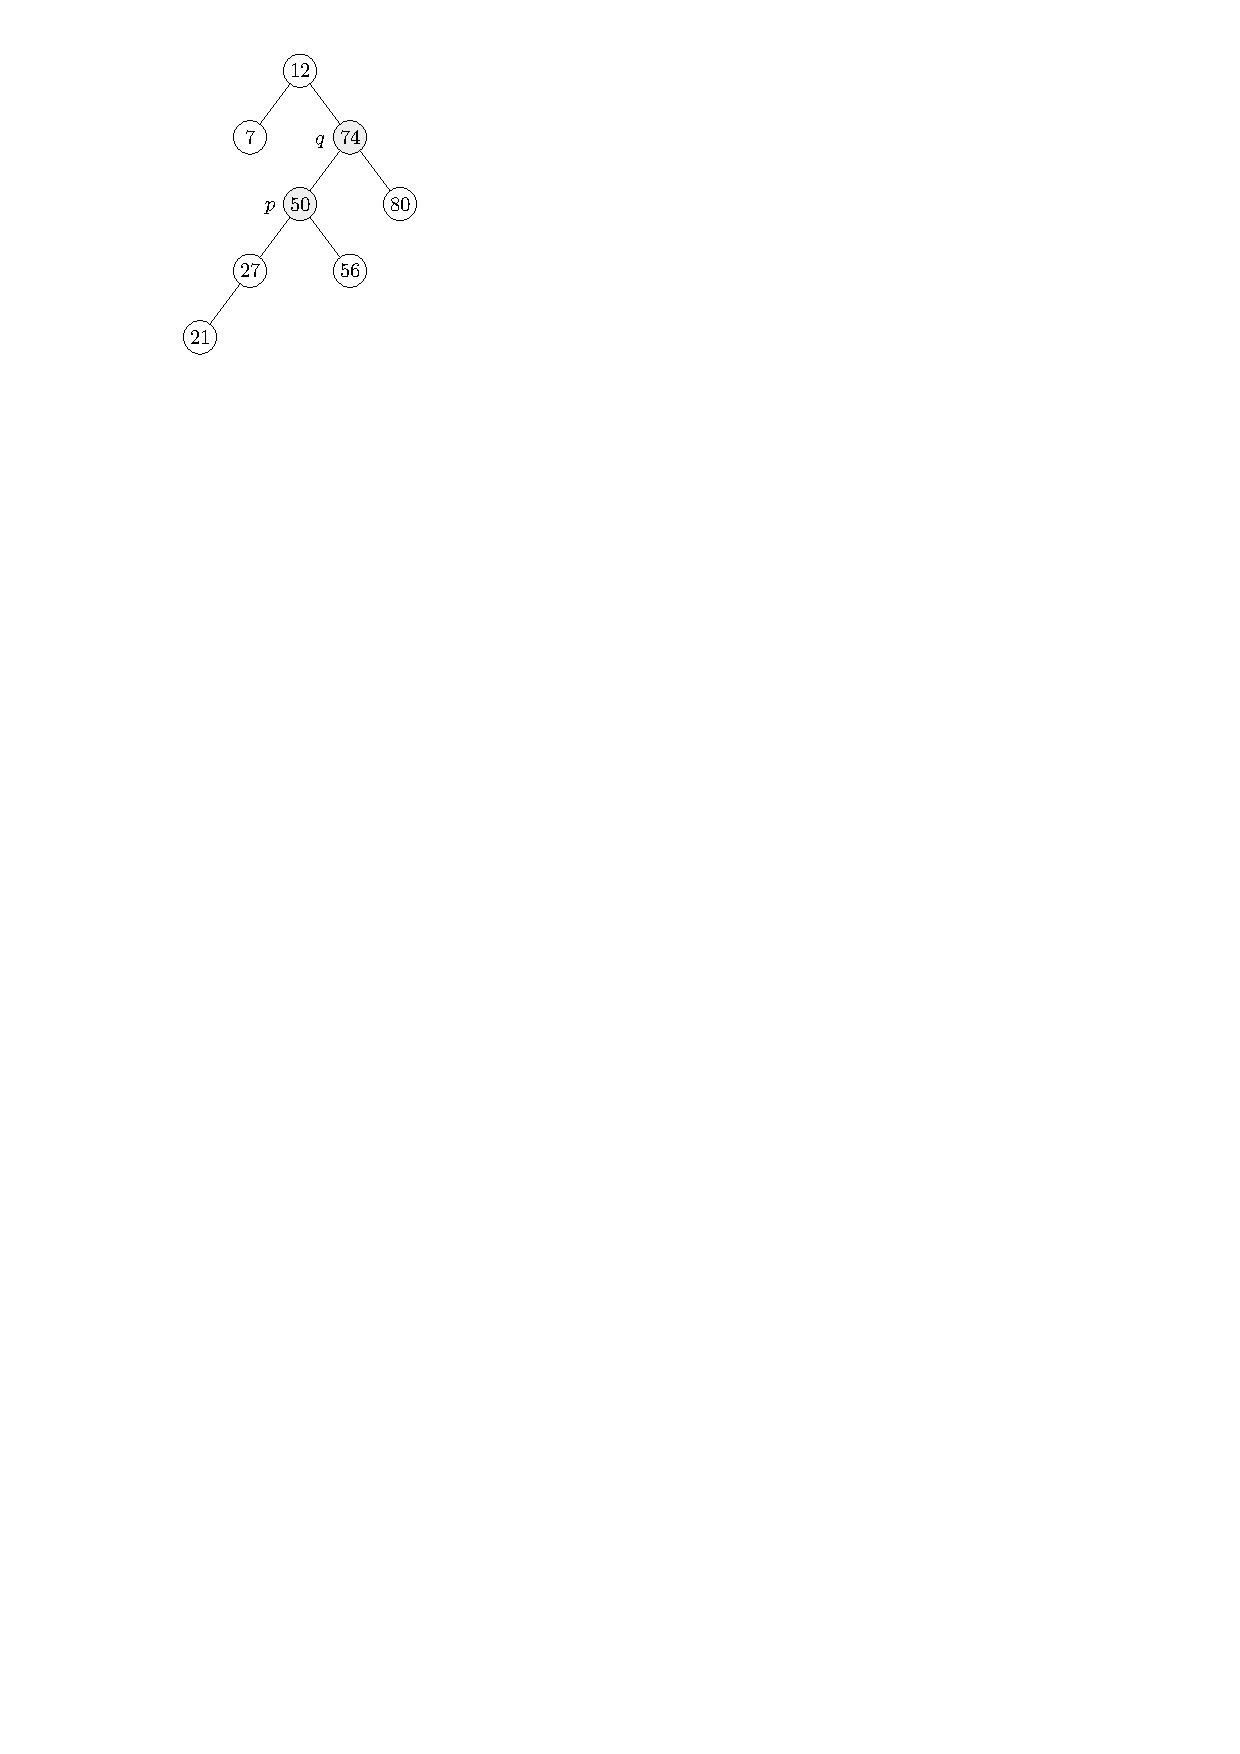
\includegraphics{rotationBoxample}
\end{Boxample}


\section{AVL trees}

These were the first self-balancing BSTs, introduced in 1962 by Adelson-Velskii and Landis. 
The \emph{balance of a node} is defined to be the difference between heights of its 
right subtree and left subtree. AVL trees adjust themselves after each insertion 
or deletion (via tricky rotations not discussed here --- see Wikipedia for gory details) so that each node has balance $0, 1$ or $-1$.

\begin{Boxample} \label{ex:avlTreeEx}
An AVL tree on the left and a non-AVL tree on the right with node balances shown below the nodes.
\begin{center}
  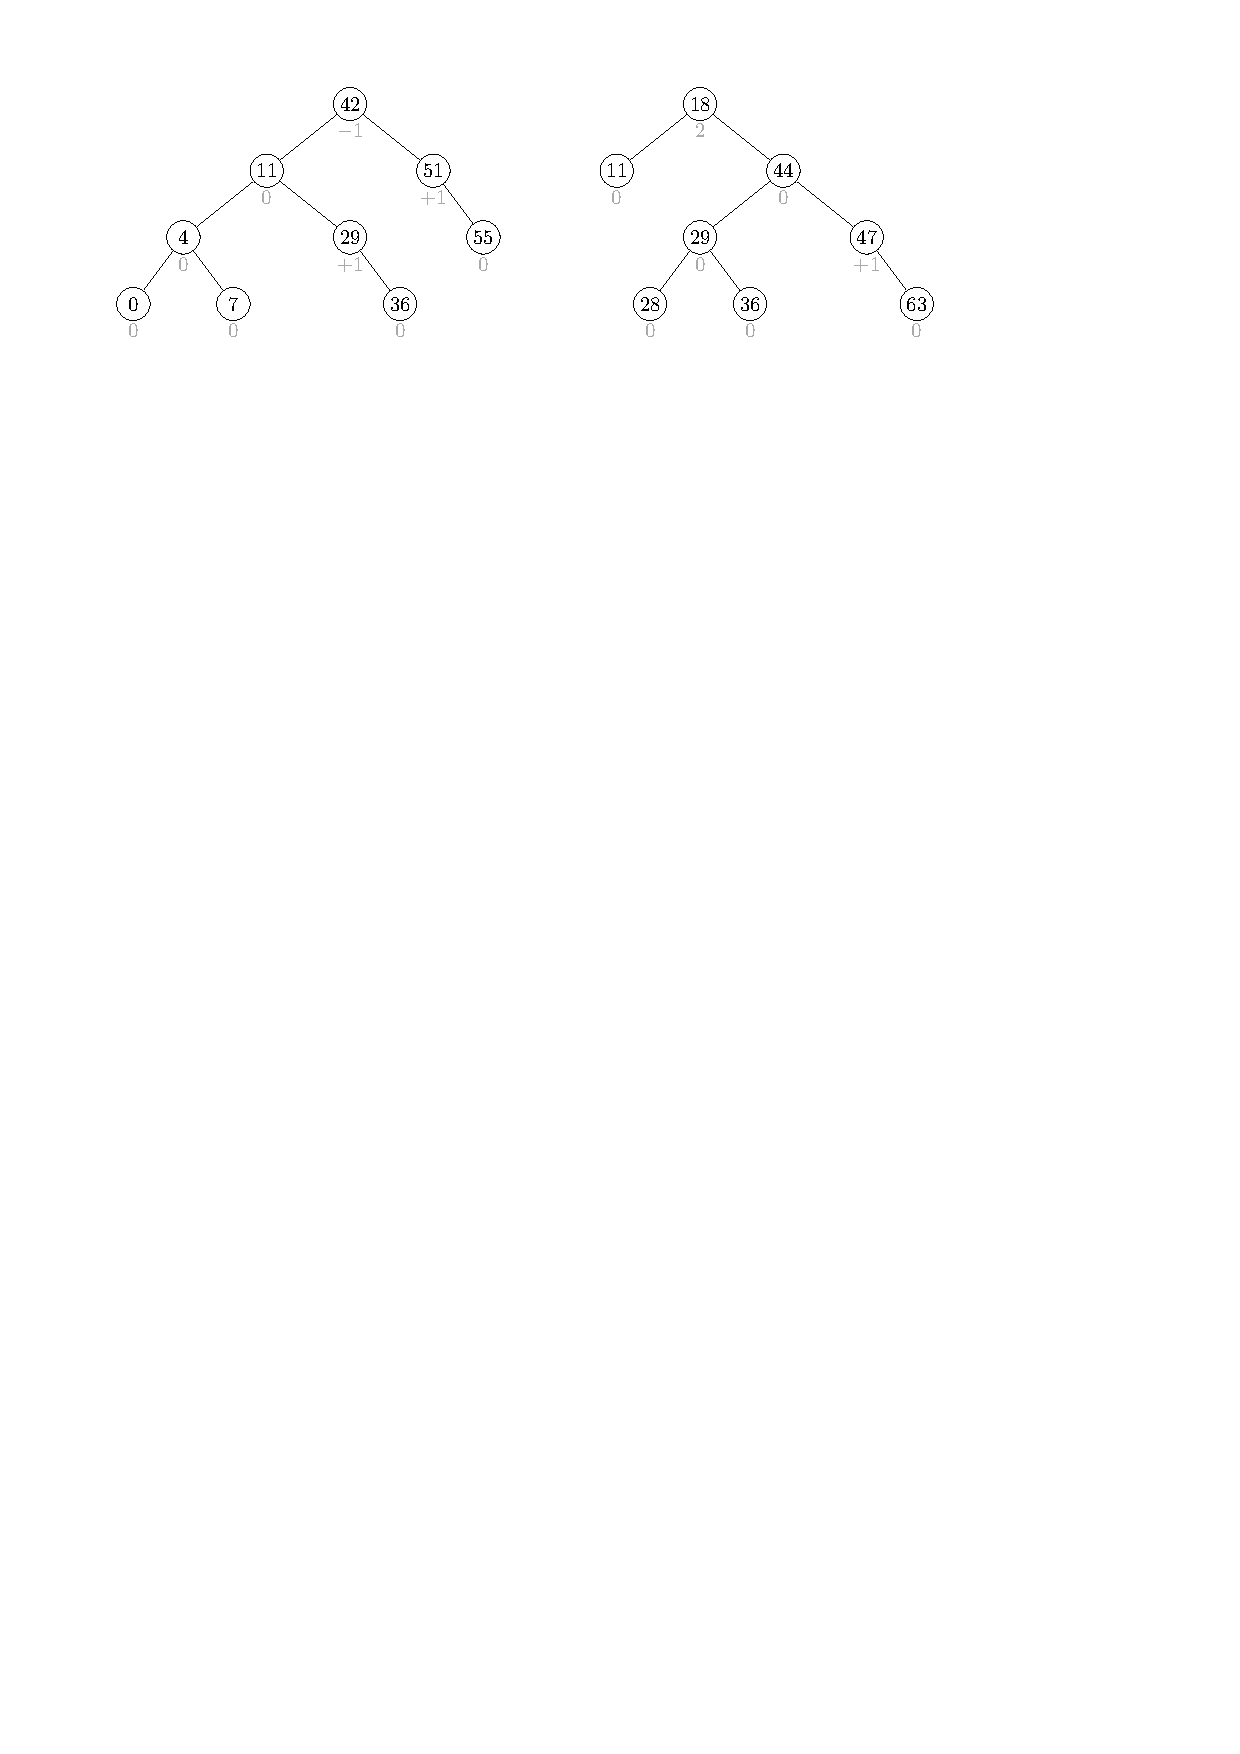
\includegraphics[width=1.0\textwidth]{avlTreeEx}
\end{center}
\end{Boxample}

\section{Height of an AVL tree}
\begin{Boxample}
An AVL tree with $n$ nodes has height at most $1.44 \lg n$, about $44\%$ more 
than optimal.

Proof: Let $A_h$ be the minimum number of nodes in a tree of height $h$. Clearly 
$A_0 = 1, A_1 = 2$. The subtrees at the root are also AVL trees of height $h-1$ or $h-2$, 
because of the balance property. Thus $A_h \geq A_{h-1} + A_{h-2} + 1$ (in fact we have equality here 
(can you see why?)). This is similar to the Fibonacci recurrence, and we know that 
$A_h \sim C \phi^h$ for some $C>0$, where $\phi = (1+\sqrt{5})/2$. 
Taking logarithms gives $h \sim \lg n / \lg \phi \approx 1.44 \lg n$. 
\end{Boxample}

\begin{Boxample}[2]
How many types of self-balancing search trees can you find (e.g. Wikipedia)?

\end{Boxample}

\section{Red-black trees}

Introduced in 1978, these have a balance condition that ensures (via tricky rotations not discussed here --- see Wikipedia for gory details) 
that the maximum depth of a leaf is no more than twice the minimum depth. 
They do this by colouring each node red or black (note that we are explicitly using external nodes), with the rules:
\begin{itemize}
\item the root is black;
\item all leaves (external nodes) are black, even when the parent is black;
\item both children of every red node are black;
\item every path from a node to a leaf contains the same number of black nodes.
\end{itemize}

\begin{Boxample} \label{ex:redblackTreeEx}
A red-black tree on the left. The BST on the right is not a red-black tree 
  because not every path from $14$ to a leaf contains the same number of black nodes.
\begin{center}
  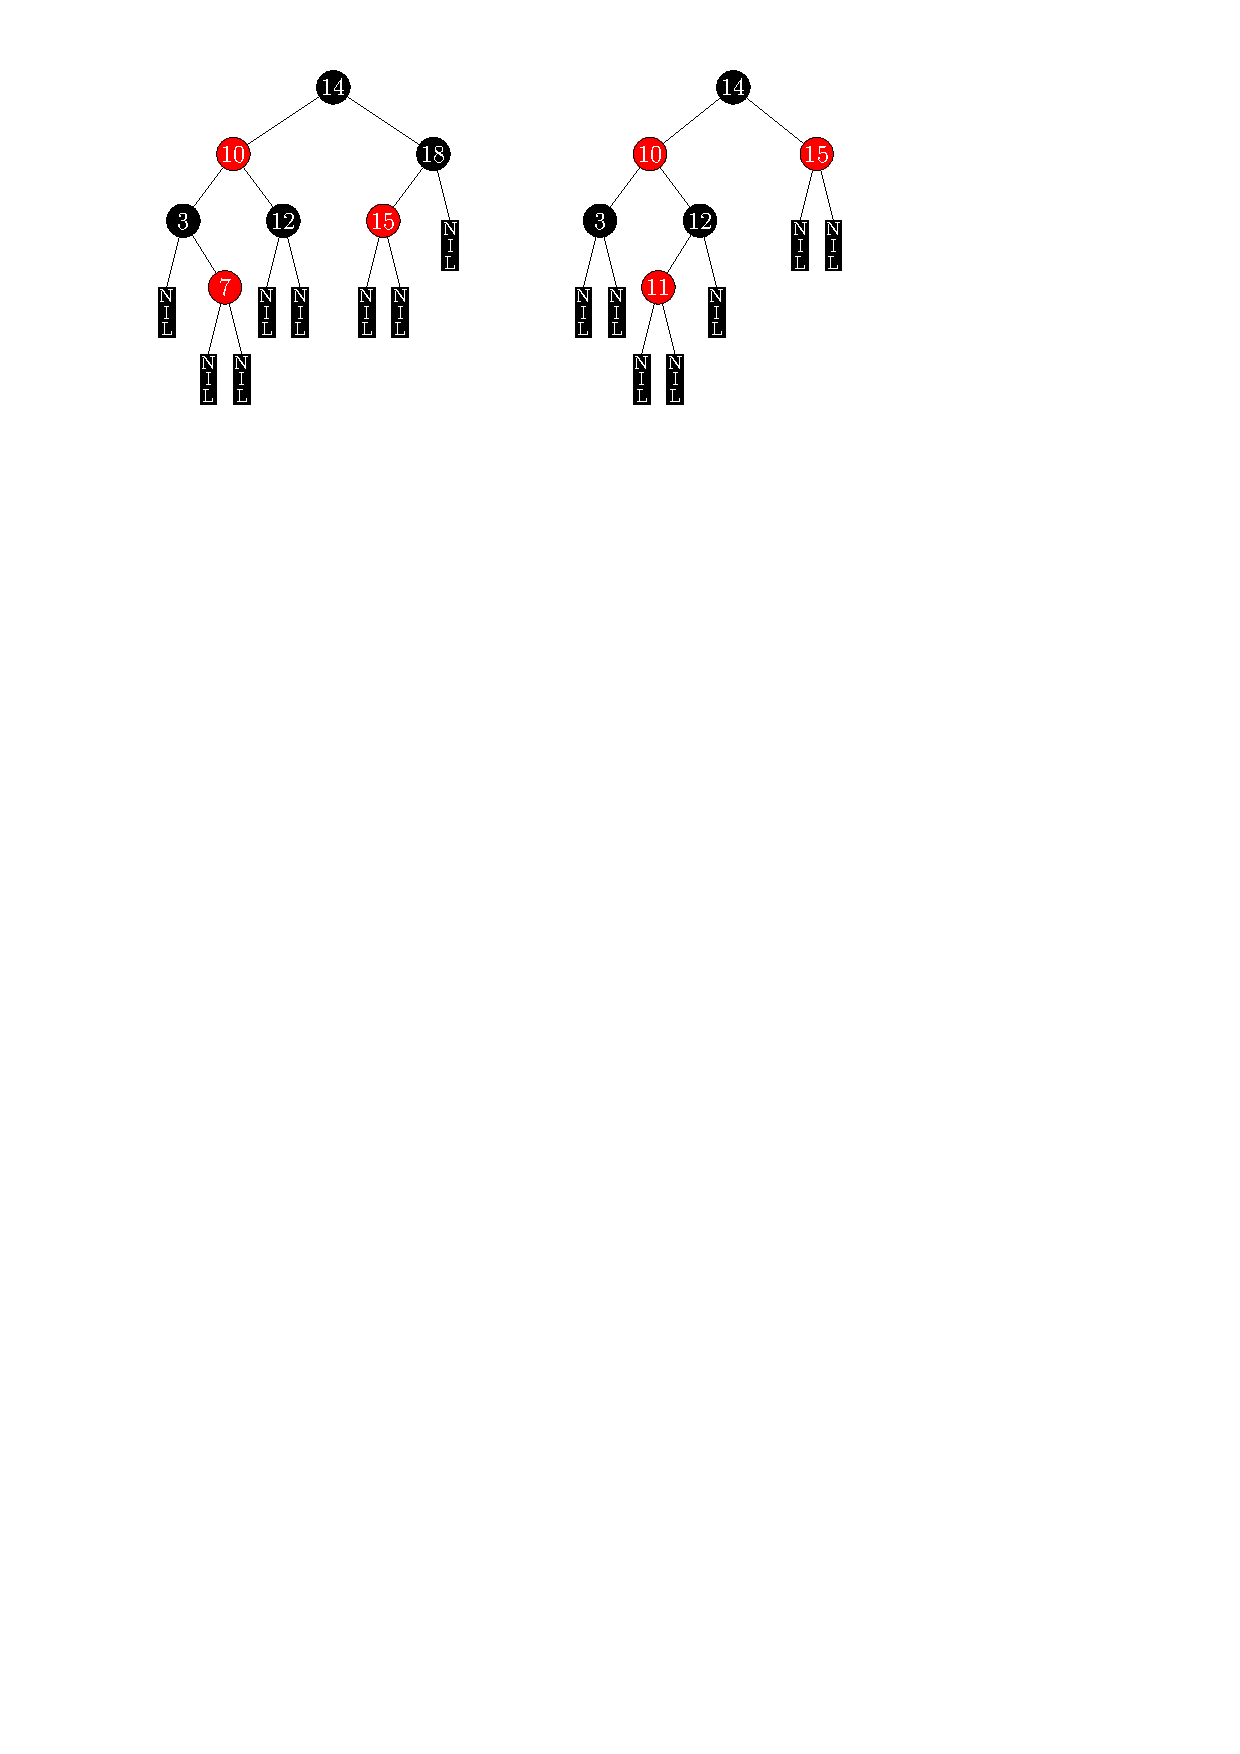
\includegraphics[width=1.0\textwidth]{redBlackEx}
\end{center}
\end{Boxample}

\section{Height of a red-black tree}
The worst case height is at most $2 \lg n$.
MCW-TODO add proof or link to it

\section{Balanced search trees in practice (Dec 2018)}
\begin{itemize}
\item Java Collections Framework uses red-black trees to implement \texttt{TreeMap}.
\item C++  uses red-black trees to implement \texttt{map}.
\item C\# uses self-balancing trees to implement \texttt{Sorted Dictionary}
\item Python uses doubly-linked lists to implement \texttt{OrderedDIct}
\end{itemize}


% \subsection{Balanced B-trees: efficiency of external search} %----------------
% \label{ss:B-tree}


\chapter{Hashing} %-----------------------------------------------------------

\begin{Definition}
A \defnfont{hash function} is a function $h$ that outputs an integer
value for each key. A \defnfont{hash table} is an array implementation of
the table ADT, where each key is mapped via a hash function to an array
index. 
\end{Definition}

There are several desirable properties of a hash function:
\begin{itemize}
\item it should be computable quickly (constant time).
\item if keys are drawn uniformly at random, then the hashed values
should be uniformly distributed. 
\item keys that are ``close" should have their hash values ``spread out". 
\end{itemize}
A hash function should be deterministic, but appear ``random" - in other 
words it should pass some statistical tests (similar to pseudorandom number generators). 

\section{Collisions}
The number of possible keys is usually enormously more than
the actual number of keys. Thus allocating an array with enough size to
fit all possible keys would be very inefficient. So hash functions are
not $1$-to-$1$; that is, two keys may be mapped to the same index -- a \defnfont{collision}. 

We need a \defnfont{collision resolution policy} to prescribe what to do when collisions occur. 
We assume the first-come-first served (FCFS) model for resolving collisions.


\subsection{Collision resolution policies}
\begin{itemize}
\item \defnfont{Open addressing} uses no extra space -- every element is stored in the hash table. 
If it gets overfull, we can reallocate space and {rehash}.
\item \defnfont{Chaining} uses an ``overflow" list for each element in 
the hash table.
%\item When a collision occurs, we can evict the occupant (LCFS), 
%evict the latecomer (FCFS) or evict the element furthest from its home location
% (\defnfont{Robin Hood} hashing).
\item When a collision occurs in open addressing, we can 
	\begin{itemize}
		\item probe nearby for a free position 
		(\defnfont{linear probing, quadratic probing});
		\item go to a ``random" position by using a second-level hash function 
		(\defnfont{double hashing}).
		%\item try a position given by a second, third, \dots hash function (this plus 
		%LCFS gives \emph{cuckoo hashing}). 
	\end{itemize}
\end{itemize}


\subsection{Collision resolution via chaining}
\begin{itemize}
\item Elements that hash to the same slot are placed in a list. The slot
contains a pointer to the head of this list. 
\item Insertion can then be done in constant time. 
\item Deletion can be done in constant time with a doubly linked list, for 
example. 
\item A drawback is the additional space overhead. Also, the distribution of 
sizes of lists turns out to be very uneven.
\end{itemize}

\begin{Boxample}
A hash table with chaining.
\begin{center}
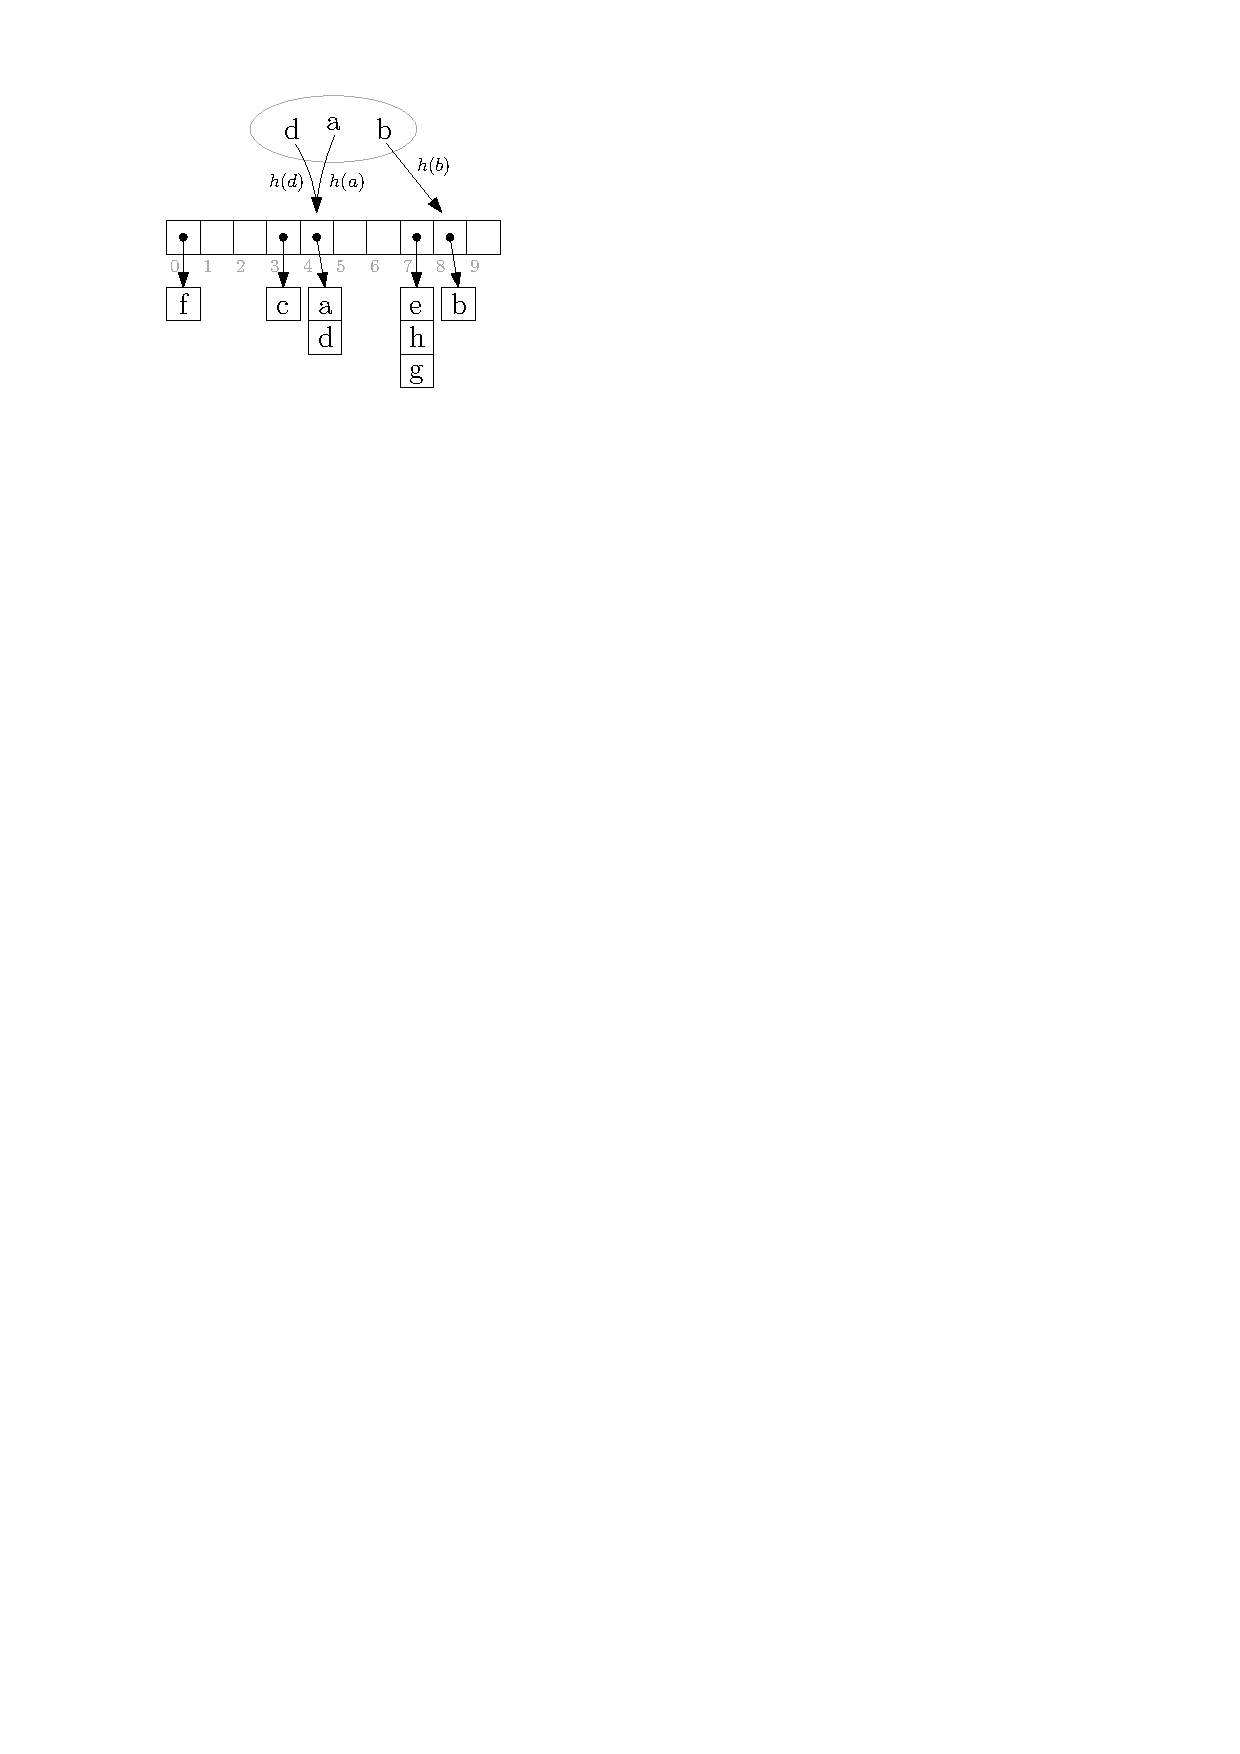
\includegraphics{hashChaining} 
\end{center}
\end{Boxample}


\subsection{Collision resolution via open addressing}
\begin{itemize}
\item Every key is stored somewhere in the array; no extra space is used.
\item If a key  $k$ hashes to a value $h(k)$ that is already occupied, 
we \defnfont{probe} (look for an empty space). 
	\begin{itemize}
		\item The most common probing method is \defnfont{linear} probing, which moves left
		 one index at a time, wrapping around if necessary, until it finds an empty 
		 address. This is easy to implement but leads to \emph{clustering}.
		\item Another method is \defnfont{double hashing}. Move to the left by a
		fixed step size $t$, wrapping around if necessary, until we find an
		empty address. The difference is that $t$ is not fixed in advance, but
		is given by a second hashing function $p(k)$.
	\end{itemize}
\end{itemize}

\begin{Boxample}
The hash table on the left uses linear probing, so $d$ is inserted two left of $h(d) = h(a)$, because $h(d)-1$ is already occupied.
The hash table on the right uses double hashing, so $d$ is moved $p(d)$ to the left of $h(d) = h(a)$. 
\begin{center}
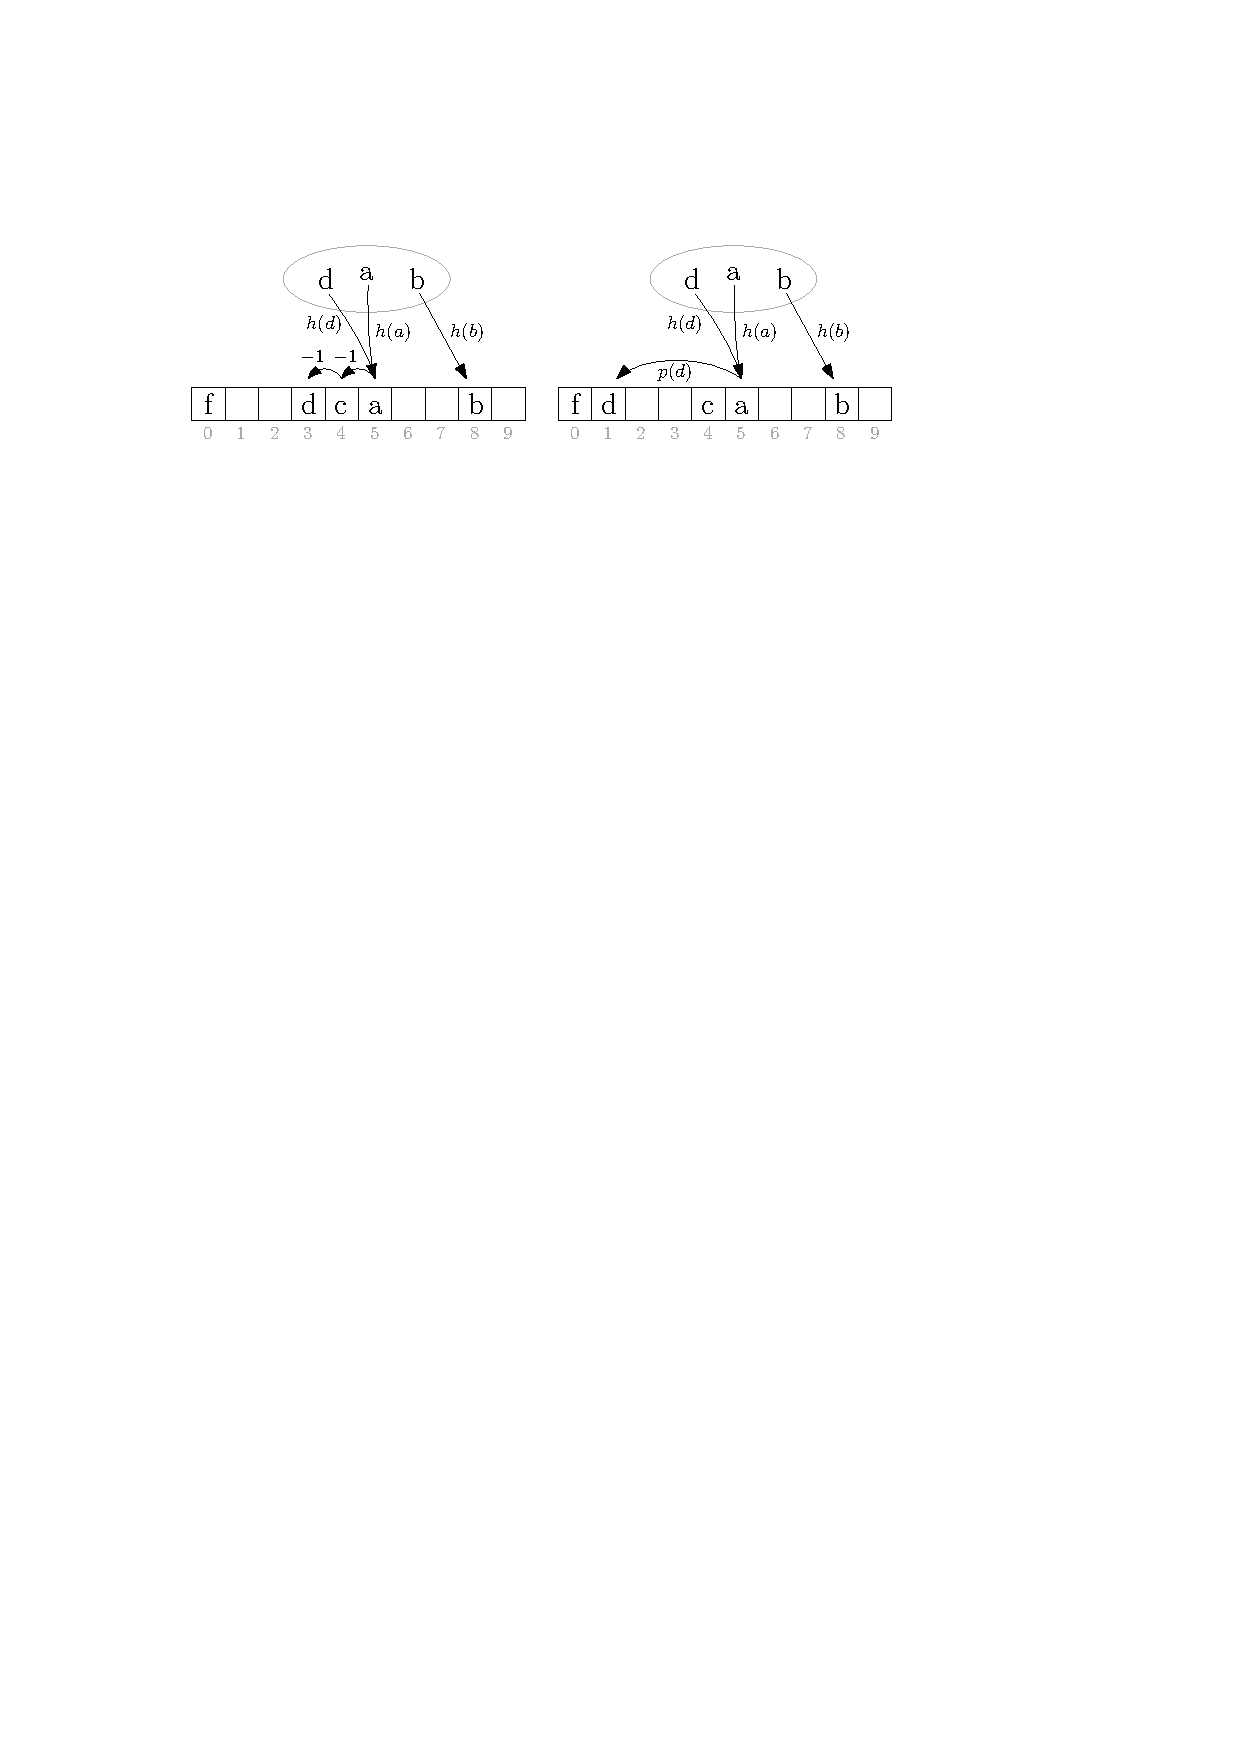
\includegraphics{hashProbing} 
\end{center}
\end{Boxample}

Linear probing is easy to implement, easier than double hashing.
However it is prone to \emph{clustering} --- large clusters of filled entries form, and this makes search times longer on average.



\section{Analysis of hashing}

We count cost by number of key comparisons/probes.

Insertion has the same cost as an unsuccessful search, provided the table 
is not full. Thus the average cost of a successful search is the average of all insertions
 needed to construct the table from empty.

We often use the \defnfont{simple uniform hashing} model. That is, each of 
the $n$ keys is equally likely to hash into any of the $m$ slots. So we are 
considering a ``balls in bins" model.

If $n$ is much smaller than $m$, collisions will be few and most slots 
will be empty. If $n$ is much larger than $m$, collisions will be many and no 
slots will be empty. The most interesting behaviour is when $m$ and $n$ are 
of comparable size. We define the \defnfont{load factor} to be $\lambda := n/m$. The results below 
will be stated in terms of $\lambda$.


\chapter{Analysis of hashing} %-------------------------------------------------

\section{Analysis of balls in bins}
Define 
$$Q(m, n) = \frac{m!}{(m-n)! m^n} = \frac{m}{m} \frac{m-1}{m} \dots 
\frac{m - n + 1}{m}.$$
Note that $Q(m,0) = 1, Q(m, n) = 0$ unless $0 \leq n \leq m$.

The probability of no collisions when $n$ balls are thrown into $m$ boxes 
uniformly at random is $Q(m, n)$. For example, $Q(366, 180) \approx 0.4487
 \times 10^{-23}$, $Q(366, 24) \approx  0.4627$. 

The expected number of balls until the first collision is equal to 
$E(m):=\sum_{n \leq m} Q(m, n)$. Note $E(365) \approx 25$.

%jo - TODO improve plots below if needed

\section{Plots of $Q(m, n)$ against $n$, $m=25,100,400,1600$}
\begin{figure}
\centering
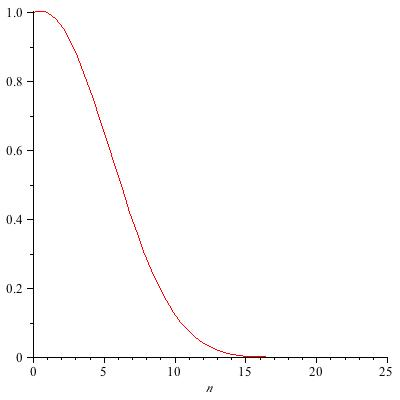
\includegraphics[width=4cm]{figs/birthday25.jpg}
$\quad$
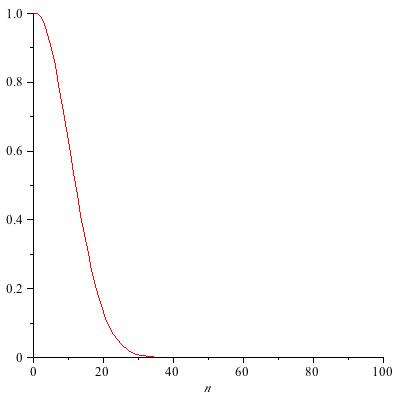
\includegraphics[width=4cm]{figs/birthday100.jpg}\\
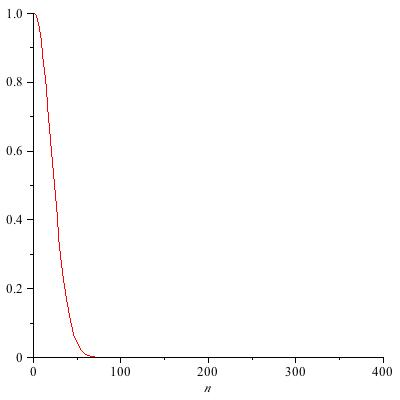
\includegraphics[width=4cm]{figs/birthday400.jpg}
$\quad$
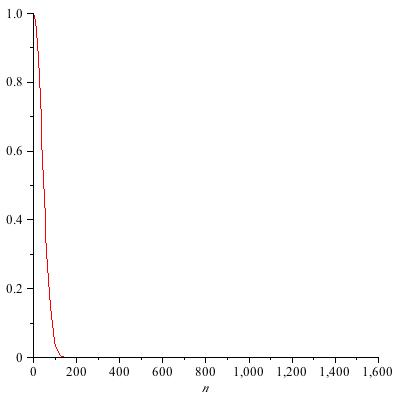
\includegraphics[width=4cm]{figs/birthday1600.jpg}
\end{figure}

\section{Results for chaining}

The worst case for searching is $\Theta(n)$, since there may be only one 
chain with all the keys. The average cost for unsuccessful search is the average list length, 
namely $\lambda$.

The average cost for successful search is then 
$$
\frac{1}{n} \sum_{k=1}^n \frac{k}{m} = \frac{n+1}{2m} \approx \lambda/2.
$$
Thus provided the load factor is kept bounded, basic operations all run in 
constant time on average. 


\section{Results for open addressing}

We assume \defnfont{uniform hashing}: each configuration of 
$n$ keys in a table of size $m$ is equally likely to occur. In other words, the 
hash function produces a random permutation of the keys, and the slots are 
probed in random order for each key.

Uniform hashing can't be implemented practically but seems to be a good 
model when double hashing is used.

It can be shown that the average cost for insertion under this 
hypothesis is $\Theta(1/(1-\lambda))$ as $m \to \infty$. 

Linear probing is not well described by the uniform hashing model 
(because of the clustering). A more detailed analysis can be done. 
The average insertion cost is $\Theta(1 + 1/(1 - \lambda)^2)$.

If the load factor is bounded away from $1$, basic operations 
run in constant time; otherwise performance will be very bad. We should resize!


\section{Extra: unsuccessful search under uniform hashing hypothesis}
\begin{itemize}
\item Let $X$ be the number of probes taken for an unsuccessful search. 
Let $p_i$ be the probability that we need to make $i+1$ probes 
(exactly $i$ probes hit an occupied cell) and let $q_i$ be the probability 
that we make at least $i+1$ probes. 
\item Then 
$E[X] = \sum_i (i+1) p_i = \sum_i q_i$.
\item For $i \geq 1$, we have
$$ q_i = \binom{n}{i}/\binom{m}{i} = \frac{n}{m} \frac{n-1}{m-1} 
\dots \frac{n - i + 1}{m - i + 1}  \leq \lambda^i.
$$
The exact value is then
$$
E[X] = \frac{1}{\binom{m}{n}} \sum_{j=0}^n \binom{(m-n)+j}{m-n} = 
\dots = \frac{1+m}{1+(1-\lambda)m}
$$
which is $\Theta(1/(1 - \lambda))$ as $\lambda \to 1$. This agrees with 
intuition.
\end{itemize}

\section{Statistics for balls in bins: some facts}
\begin{itemize}
\item When do we expect the first collision? This is the 
{birthday problem}. Answer: $E(m) \approx \sqrt{\pi m/2} + 2/3$.
So collisions happen even in fairly sparse tables.
\item When do we expect all boxes to be nonempty? This is the 
{coupon collector problem}. Answer: after about $m \log m$ balls. 
It takes a long time to use all lists when chaining.
\item What proportion of boxes are expected to be empty when $n$ is $\Theta(m)$? 
Answer: $e^{-\lambda}$. Many of the lists are just wasted space even for 
pretty full tables.
\item When $m$ is $\Theta(n)$, what is the expected maximum number of balls in a box? 
Answer: about $(\log n)/(\log \log n)$. Some of the lists may be fairly long. 
\item The analysis that gives these results is beyond this course. See lecturer for 
references.
\end{itemize}

\section{Hashing in practice (Dec 2018)}
\begin{itemize}
\item Java Collections Framework uses chaining to implement \texttt{HashMap}, resizing when $\lambda > 0.75$, and table size a power of $2$.
\item C++  uses chaining to implement \texttt{unordered\_map}, resizing when $\lambda >1$, and prime table size.
\item C\# uses chaining, resizing when $\lambda >1$, and prime table size.
\item Python uses open addressing, resizing when $\lambda>0.66$, and table size a power of $2$.
\end{itemize}





\chapter{Universal Hashing} %-------------------------------------------------


Hash functions must be deterministic, but we don't want  to let users know what they are. 
However, they can often guess. As with quicksort, a malicious user can submit input data that makes the 
algorithm run an unreasonably long time, which can cause security and performance problems.

\begin{Boxample}[4]
\item Java String \texttt{hashcode} computes the address of a string, say 
$s=s[0]\cdots s[n-1]$ using integer arithmetic via the formula 
$s[0]*31^{n-1} + s[1]*31^{n-2} + ... + s[n-1]$. Can you find two 2-character strings with the same hashcode? 
Why might this cause a problem in practice?
\end{Boxample}


A nice way to use randomization is to choose the hash function at runtime randomly from a family of hash functions.
Ideally,   the probability of a collision between two elements is only $1/m$, which is what a random guess would yield, so malicious users cannot 
force collisions. A family satisfying this is called \defnfont{universal}.

More formally, if $F$ is a family of hash functions then for any keys $k\neq k'$, we have
$$
\frac{1}{|F|} \left| h\in F : h(k) = h(k') \right| \leq \frac{1}{m}.
$$

\begin{Boxample}[6]
One way of constructing such an $F$ is to take a prime $p\geq m$  and for $0<a <p, 0\leq b < p$ define 
$$h_{ab}(x) = ax+b \mod p \mod m.$$ Prove that this is a universal family.

\end{Boxample}




Here is a summary of the results so far on table implementations.


\begin{table}[htb] 
\caption{Worst case running time (asymptotic order)} 
\centerline{
\begin{tabular}{|c|c|c|c|c|} \hline 
Data structure & Insert & Delete & Find & Traverse \\
\hline
Unsorted list (array) & $1$ & $n$ & $n$  & $n$  \\
Unsorted list (pointer) & $1$ & $n$ & $n$ &  $n$ \\
Sorted list (array)& $n$  & $n$  & $\log n$ & $n$\\
Sorted list (pointer)& $n$ & $n$ & $n$ & $n$ \\
Binary search tree & $n$ & $n$ & $n$ & $n$  \\
Balanced BST & $\log n$ & $\log n$ & $\log n$ & $n$ \\
Hash table & $n$ & $n$ & $n$ & $n$ \\
\hline
\end{tabular}}
\end{table}

\begin{Boxample}[6]
If we want to print out all items of a table in sorted order, what is the best data structure?
If we don't mind an occasional long wait and mostly do lookups, which is best?
If we do a lot of insertions and deletions and few lookups, and are risk-averse, which is best?
\end{Boxample}









